\chapter{Revisão Bibliográfica}
\label{sec:revbib}

Este capítulo apresentou o referencial teórico que embasou o problema e a solução desenvolvidos. A primeira parte situou o leitor no contexto institucional em que o problema ocorreu: o IFNMG -- Campus Salinas e a forma como instituições de ensino lidaram com a gestão de espaços físicos. A segunda parte apresentou os trabalhos relacionados, descrevendo iniciativas semelhantes já documentadas na literatura e identificando em que pontos o presente trabalho se distinguiu delas. A terceira parte reuniu os conceitos técnicos que fundamentaram o desenvolvimento do sistema web, cobrindo engenharia de software, modelagem com UML, banco de dados, controle de acesso, arquitetura web, usabilidade e testes.

%-----------------------------------
\subsection{Contexto Institucional}
\label{sec:contexto}

Esta seção descreve o IFNMG -- Campus Salinas e o funcionamento dos seus espaços físicos e apresenta o que a literatura registra sobre gestão de espaços em ambientes acadêmicos.

%-----------------------------------
\subsubsection{O IFNMG e o Campus Salinas}
\label{sec:ifnmg}

O Instituto Federal de Educação, Ciência e Tecnologia do Norte de Minas Gerais (IFNMG) é uma autarquia federal criada pela Lei n.º 11.892, de 29 de dezembro de 2008, que reorganizou a Rede Federal de Educação Profissional, Científica e Tecnológica no Brasil. Conforme seu Plano de Desenvolvimento Institucional, o IFNMG tem por missão promover educação profissional, científica e tecnológica por meio do ensino, da pesquisa e da extensão, com vistas à formação humana integral e ao desenvolvimento regional \cite{ifnmg2024pdi}.

O Campus Salinas integra a rede do IFNMG e oferta cursos em diferentes níveis e modalidades, entre eles o Bacharelado em Sistemas de Informação, no âmbito do qual este trabalho está inserido. Para o funcionamento dessas atividades acadêmicas, o campus dispõe de laboratórios de informática e outras salas especiais cujo uso é compartilhado por diferentes turmas e docentes ao longo do período letivo, o que exige mecanismos de organização e controle sobre a ocupação desses espaços.

A natureza dos institutos federais agrava esse desafio. Ao contrário de instituições que ofertam um único tipo de curso, os IFs atendem simultaneamente a turmas de educação técnica integrada ao ensino médio, cursos técnicos subsequentes e cursos de nível superior, todos com horários distintos e, em muitos casos, disputando os mesmos laboratórios. Um laboratório de informática, por exemplo, pode ser utilizado em horários diferentes para aulas de disciplinas técnicas, para disciplinas do bacharelado e para atividades de extensão, o que torna a gestão manual da disponibilidade um trabalho de complexidade operacional \cite{ifnmg2024pdi}.

%-----------------------------------
\subsubsection{A Gestão de Espaços em Instituições de Ensino}
\label{sec:gestao}

A gestão dos espaços físicos em instituições de ensino inclui o planejamento do uso, o controle de disponibilidade, o registro de ocupações e o acompanhamento de como os recursos são efetivamente utilizados. Quando esses mecanismos não existem ou são precários, o resultado é a subutilização dos espaços e a dificuldade de responder a demandas concretas dos usuários.

Esse cenário se repete em outras instituições públicas de ensino, como mostram os trabalhos de \citeonline{cruz2023gestao} e \citeonline{nascimento2020reservas}, discutidos na Seção~\ref{sec:trabrel}.

%-----------------------------------
\subsection{Trabalhos Relacionados}
\label{sec:trabrel}

Esta seção apresenta trabalhos e soluções que trataram de problemas semelhantes ao abordado nesta pesquisa, seja pelo diagnóstico da gestão de espaços em instituições federais de ensino, seja pelo desenvolvimento de sistemas de reserva em ambientes acadêmicos, seja pela oferta de ferramentas de mercado para a reserva de espaços. A análise desses trabalhos e soluções permite situar a presente proposta em relação ao que já foi produzido e identificar os aspectos que a diferenciam.

%-----------------------------------
\subsubsection{Soluções Existentes de Reserva de Espaços}
\label{sec:relsoftwares}

Além dos trabalhos acadêmicos, foram analisadas soluções de software já disponíveis para a reserva de espaços, com o objetivo de verificar se alguma delas resolveria o problema do Campus Salinas sem a necessidade de desenvolvimento de um sistema específico. A análise concentrou-se em duas plataformas comerciais representativas: o Skedda e o Microsoft Bookings.

O Skedda é uma plataforma web dedicada à reserva de espaços físicos, como salas, escritórios e laboratórios, que oferece autoatendimento aos usuários, definição de regras de reserva e visualização de disponibilidade em formato de agenda \cite{skedda2025}. O Microsoft Bookings, integrante do pacote Microsoft 365, é voltado ao agendamento de compromissos e ao gerenciamento de calendários, com reserva de recursos por meio de caixas de correio associadas a salas \cite{microsoft2025bookings}. As duas plataformas possuem funções presentes também no sistema proposto: consulta de disponibilidade, solicitação de reserva pelo próprio usuário e notificação das partes envolvidas.

Nenhuma das duas, contudo, resolve o problema central do campus: fazer a disponibilidade refletir a grade de horários institucional. Como não importam as planilhas de horários, a ocupação das aulas teria de ser cadastrada manualmente a cada semestre, exatamente o retrabalho que motiva esta proposta. Além disso, são soluções proprietárias, pagas por assinatura e hospedadas em servidores externos, o que gera custos recorrentes e reduz o controle da instituição sobre os próprios dados.

%-----------------------------------
\subsubsection{Gestão de Laboratórios no IFNMG Campus Almenara}
\label{sec:relcaio1}

\citeonline{cruz2023gestao} conduziram uma pesquisa de campo no IFNMG Campus Almenara com o objetivo de analisar a utilização dos espaços e equipamentos dos laboratórios educacionais daquela unidade. O estudo adotou abordagem qualitativa e quantitativa, com coleta de dados por meio de questionários aplicados a servidores e docentes do campus. Os resultados revelaram que a gestão dos laboratórios ocorre de forma informal, baseada exclusivamente em reservas pontuais feitas com antecedência, sem planejamento oficial permanente e sem qualquer mecanismo para medir o desempenho ou a eficiência no uso desses espaços.

O trabalho de \citeonline{cruz2023gestao} é relevante para esta pesquisa porque documenta, em outro campus do IFNMG, uma dificuldade semelhante à observada em Salinas. Os autores concentram-se no diagnóstico e não apresentam uma solução de software. Neste trabalho, essa lacuna é abordada com um sistema que importa os horários das aulas, controla a disponibilidade e registra o histórico de uso dos espaços.

%-----------------------------------
\subsubsection{Sistema Web de Reservas na UESPI -- Parnaíba}
\label{sec:relcaio2}

\citeonline{nascimento2020reservas} desenvolveram um sistema web para controlar pedidos de reservas de recursos físicos na Universidade Estadual do Piauí, Campus Parnaíba. O contexto era semelhante ao do presente trabalho: as reservas de espaços e equipamentos eram registradas manualmente por servidores em uma agenda digital, e a demanda tornava o processo oneroso e sujeito a falhas. A solução desenvolvida pelos autores automatizou o controle das solicitações, disponibilizou a interface para os usuários da instituição e obteve avaliação positiva quanto à satisfação dos usuários com o sistema.

O trabalho de \citeonline{nascimento2020reservas} apresenta uma aplicação de reservas para uma instituição de ensino e relata avaliação positiva dos usuários. O sistema deste trabalho trata do mesmo tipo de demanda, mas acrescenta a importação das planilhas de horários institucionais, com possibilidade de reimportação ou ajuste pontual ao longo do semestre. Também oferece consulta pública da ocupação, sem autenticação, e relatórios de uso dos espaços, recursos que não são descritos no trabalho referenciado. A Tabela~\ref{tab:comparativo} resume essa comparação.

\begin{table}[!htb]
	\centering
	\caption{Comparação entre o sistema proposto e os trabalhos relacionados}
	\begin{tabular}{@{}>{\raggedright\arraybackslash}p{5.6cm}cccc@{}}
	\hline
		\textbf{Funcionalidade} & \textbf{Skedda} & \textbf{\begin{tabular}[c]{@{}c@{}}MS\\ Bookings\end{tabular}} & \textbf{\begin{tabular}[c]{@{}c@{}}Nascimento, Rios\\ e Baluz (2020)\end{tabular}} & \textbf{\begin{tabular}[c]{@{}c@{}}Este\\ trabalho\end{tabular}} \\ \hline
		Solicitação de reserva pelo próprio usuário & $\checkmark$ & $\checkmark$ & $\checkmark$ & $\checkmark$ \\
		Aprovação das solicitações & $\checkmark$ & P & $\checkmark$ & $\checkmark$ \\
		Notificações automáticas & $\checkmark$ & $\checkmark$ & $\checkmark$ & $\checkmark$ \\
		Consulta pública, sem login & $\checkmark$ & P & $\times$ & $\checkmark$ \\
		Importação da grade de horários institucional & $\times$ & $\times$ & $\times$ & $\checkmark$ \\
		Relatórios de uso dos espaços & $\checkmark$ & $\checkmark$ & -- & $\checkmark$ \\
		Sem custo de assinatura & $\times$ & $\times$ & $\checkmark$ & $\checkmark$ \\ \hline
	\end{tabular}
	\caption*{\footnotesize Legenda: $\checkmark$ atende; P atende parcialmente; $\times$ não atende; -- não informado. \citeonline{cruz2023gestao} não consta na comparação por se tratar de estudo diagnóstico, sem sistema desenvolvido.\\ Fonte: Elaborado pelo autor (2026).}
	\label{tab:comparativo}
\end{table}

%-----------------------------------
\subsection{Fundamentação Tecnológica}
\label{sec:fundtec}

Esta seção apresenta os conceitos técnicos que embasam o sistema proposto: engenharia de software, UML, banco de dados, controle de acesso, arquitetura web, o \textit{framework} Django, usabilidade e testes.

%-----------------------------------
\subsubsection{Engenharia de Software}
\label{sec:engsw}

\citeonline{sommerville2018} define software como programas de computador e documentação associada, que pode ser desenvolvido para um cliente específico ou para o mercado em geral. A engenharia de software é a disciplina que se ocupa de todos os aspectos da produção de software, desde a especificação inicial do sistema até as necessidades de manutenção após a sua implantação. Deste campo, este trabalho se apoia diretamente em dois pontos: a especificação de requisitos e os atributos de qualidade que orientam as decisões de projeto.

Um conceito central dessa disciplina é a especificação de requisitos. \citeonline{sommerville2018} distingue os requisitos funcionais dos não funcionais: os primeiros descrevem as funções que o sistema deve executar e como deve se comportar em situações específicas; os segundos estabelecem restrições ao sistema, como desempenho, segurança e disponibilidade.

\citeonline{sommerville2018} também descreve atributos que um sistema de software profissional precisa apresentar para ser considerado de boa qualidade: manutenibilidade, ou seja, a capacidade de evoluir para atender a necessidades futuras; confiabilidade e segurança, que inclui comportamento correto e proteção contra falhas e acessos indevidos; eficiência, que diz respeito ao uso criterioso dos recursos de hardware; e aceitabilidade, que significa ser compreensível e compatível com o que os usuários esperam.

%-----------------------------------
\subsubsection{Modelagem de Sistemas com UML}
\label{sec:uml}

A \textit{Unified Modeling Language} (UML) é uma linguagem de modelagem padronizada para especificar, visualizar e documentar sistemas de software orientados a objetos \cite{bezerra2007}. \citeonline{bezerra2007} esclarece que a UML não é uma metodologia de desenvolvimento, mas uma notação que pode ser adotada em conjunto com diferentes processos. Ela oferece um conjunto de diagramas que representam aspectos distintos do sistema, como a sua estrutura estática e o seu comportamento dinâmico.

O diagrama de casos de uso descreve as funcionalidades do sistema do ponto de vista de quem interage com ele. Seus elementos são os atores, que representam papéis desempenhados por usuários ou sistemas externos, e os casos de uso, que representam as funções oferecidas. Um ator pode especializar outro por generalização, herdando suas interações. Entre casos de uso, a relação «include» indica um comportamento sempre incorporado ao caso base, e a relação «extend», um comportamento opcional que o estende \cite{bezerra2007}.

O diagrama de classes representa a estrutura estática do sistema. Cada classe reúne atributos e operações, e as associações entre classes indicam, pela multiplicidade, quantos objetos de uma se relacionam com os da outra. A composição é uma associação em que a parte não existe sem o todo \cite{larman2007}.

O diagrama de sequência representa o comportamento dinâmico, mostrando as mensagens trocadas entre os participantes ao longo do tempo. Cada participante tem uma linha de vida vertical, as mensagens aparecem de cima para baixo na ordem em que ocorrem, e o fragmento \textit{alt} representa caminhos alternativos condicionados a uma guarda \cite{larman2007}.

\citeonline{larman2007} destaca que a modelagem com UML permite registrar e comunicar decisões de projeto de forma visual antes de qualquer implementação, o que facilita o alinhamento entre desenvolvedores e demais partes envolvidas.
%-----------------------------------
\subsubsection{Banco de Dados Relacional}
\label{sec:bd}

Um banco de dados é uma coleção organizada de dados inter-relacionados, gerenciada por um sistema que permite armazená-los, recuperá-los e manipulá-los com eficiência \cite{heuser2009}. \citeonline{heuser2009} apresenta o modelo entidade-relacionamento como a principal ferramenta para o projeto conceitual de bancos de dados, por permitir representar as entidades do domínio e os vínculos entre elas antes de definir como os dados serão fisicamente armazenados.

O modelo relacional organiza os dados em tabelas formadas por linhas e colunas, onde cada tabela representa uma entidade e cada linha, um registro dessa entidade. A integridade dos dados é assegurada por restrições como chaves primárias e estrangeiras, que garantem a unicidade dos registros e os vínculos entre tabelas \cite{silberschatz2012}. \citeonline{heuser2009} também descreve o processo de normalização, pelo qual o esquema relacional é reorganizado para eliminar redundâncias e anomalias de atualização. Um banco de dados normalizado garante que cada informação seja armazenada em um único lugar, reduzindo o risco de inconsistências quando os dados precisam ser modificados.

\citeonline{silberschatz2012} definem um sistema gerenciador de banco de dados (SGBD) como um conjunto de programas que permite criar, manter e acessar um banco de dados. Os autores também descrevem a linguagem SQL (\textit{Structured Query Language}) como o padrão para definir esquemas, inserir dados e realizar consultas em bancos de dados relacionais. A SQL combina uma linguagem de definição de dados, para criar e alterar tabelas e restrições, com uma linguagem de manipulação de dados, para inserir, atualizar, remover e consultar registros. Para o sistema proposto, o uso de um SGBD relacional é adequado porque os dados a serem gerenciados (espaços físicos, horários, usuários, solicitações de reserva) têm estrutura bem definida e mantêm entre si relacionamentos que o modelo relacional representa com precisão.

Entre os SGBDs relacionais disponíveis, o PostgreSQL é um sistema de código aberto com mais de três décadas de desenvolvimento, reconhecido pela conformidade com o padrão SQL e pela robustez no tratamento de transações. Ele garante as propriedades ACID (atomicidade, consistência, isolamento e durabilidade), oferece suporte a tipos de dados avançados, controle de concorrência multiversão (MVCC) e recursos como busca textual e integridade referencial, características que o tornam adequado a aplicações que exigem consistência e confiabilidade no armazenamento dos dados \cite{postgresql2024}.

%-----------------------------------
\subsubsection{Controle de Acesso Baseado em Papéis}
\label{sec:rbac}

O controle de acesso define quais usuários têm permissão para executar quais operações em um sistema. Entre os modelos existentes, o \textit{Role-Based Access Control} (RBAC) proposto por \citeonline{sandhu1996rbac} é amplamente adotado em sistemas de informação institucionais.

No modelo RBAC, os direitos de acesso são associados a papéis, e os usuários adquirem esses direitos ao serem atribuídos a um ou mais papéis. \citeonline{sandhu1996rbac} descrevem que essa abordagem simplifica a administração, pois as permissões são definidas no nível do papel e não para cada usuário individualmente. Quando as responsabilidades de um usuário mudam, basta alterar a sua atribuição de papéis, sem necessidade de revisar cada permissão específica.

\citeonline{sandhu1996rbac} definem quatro modelos de referência que compõem a família RBAC. O RBAC0, o modelo base, define os elementos fundamentais: usuários, papéis, permissões e sessões, onde uma sessão corresponde a um período de atividade de um usuário dentro de um subconjunto dos seus papéis. O RBAC1 estende o modelo base com hierarquias de papéis, permitindo que papéis mais abrangentes herdem as permissões de papéis subordinados. O RBAC2 acrescenta restrições ao RBAC0, incluindo o conceito de separação de obrigações, pelo qual um usuário não pode acumular simultaneamente papéis conflitantes. O RBAC3 combina hierarquias e restrições, reunindo as características dos modelos anteriores.

O sistema proposto segue o RBAC0 com restrições típicas do RBAC2, sem hierarquia de papéis. As restrições adotadas são a cardinalidade, pela qual cada usuário tem no máximo um perfil, e a reserva de permissões administrativas, que não podem ser atribuídas a nenhum perfil. No padrão NIST para RBAC, essa configuração corresponde ao \textit{Core RBAC} com restrição de cardinalidade \cite{ferraiolo2001nist}. Como cada usuário tem um único perfil, a separação de obrigações entre papéis conflitantes não se aplica.

Duas regras do sistema complementam o modelo por papéis. A primeira trata de quem pode atribuir perfis: um usuário só atribui um perfil se já tiver todas as permissões dele, questão estudada pelo RBAC administrativo \cite{sandhu1999arbac97}. A segunda considera o vínculo do usuário com o registro, e não só o perfil: o docente de uma aula pode cancelar as ocorrências dela, e disciplinas e turmas ficam limitadas ao escopo do docente. Esse tipo de verificação se aproxima do controle por atributos, combinado ao RBAC em modelos híbridos \cite{kuhn2010attributes}.

%-----------------------------------
\subsubsection{Desenvolvimento Web e Arquitetura de Software}
\label{sec:web}

Um sistema web é uma aplicação de software acessada por meio de um navegador, que utiliza a infraestrutura da internet para a comunicação entre clientes e servidores. \citeonline{tanenbaum2011} descrevem a \textit{World Wide Web} como um sistema de documentos interconectados distribuídos pela internet, baseado no protocolo HTTP para a troca de informações. Esse modelo de comunicação é a base sobre a qual sistemas web são construídos.

Do ponto de vista arquitetural, \citeonline{laudon2014} descrevem que sistemas de informação baseados na web se organizam tipicamente em três camadas: a de apresentação, responsável pela interface com o usuário no navegador; a de aplicação, onde ficam as regras de negócio; e a de dados, onde as informações são armazenadas. No sistema proposto, essa divisão separa as telas, as regras de reserva e o armazenamento dos registros, evitando que uma alteração visual exija mudanças diretas no esquema do banco de dados.

\citeonline{tanenbaum2011} descrevem o protocolo HTTP como uma especificação sem estado (\textit{stateless}), o que significa que cada requisição do cliente ao servidor é tratada de forma independente, sem que o servidor retenha informações sobre interações anteriores. Essa característica simplifica a arquitetura dos servidores web, mas exige que o estado da aplicação, como a sessão do usuário autenticado, seja gerenciado explicitamente pela camada de aplicação, por meio de mecanismos como \textit{tokens} de autenticação.

\citeonline{laudon2014} também apontam que sistemas web têm a vantagem de não exigir instalação de software no dispositivo do usuário: basta um navegador com acesso à internet para que o sistema esteja disponível. Isso reduz os custos de implantação, elimina problemas de compatibilidade entre sistemas operacionais e centraliza a manutenção no servidor, onde atualizações passam a valer imediatamente para todos os usuários. No caso do sistema proposto, essa característica é relevante porque os docentes do campus utilizam dispositivos variados e não dependem de nenhuma configuração específica para acessar a plataforma de reservas.

Para o sistema proposto, a arquitetura em três camadas é adequada porque isola a interface utilizada pelos docentes da lógica que controla as reservas e da base de dados onde os registros são mantidos. Na prática, essa separação é implementada por meio de um \textit{framework} web, que fornece a estrutura de código e os mecanismos de comunicação entre as camadas, reduzindo o trabalho de infraestrutura e permitindo que o desenvolvimento se concentre nas regras de negócio da aplicação. O padrão arquitetural adotado pelo \textit{framework} escolhido para este sistema é detalhado na seção a seguir.

%-----------------------------------
\subsubsection{Padrões Arquiteturais para Aplicações Web: MVC e MTV}
\label{sec:mvc_mtv}

O padrão \textit{Model-View-Controller} (MVC) é uma abordagem arquitetural consolidada para organizar o código de aplicações interativas em três componentes com responsabilidades bem delimitadas. O \textit{Model} gerencia os dados e as regras de negócio da aplicação. A \textit{View} é responsável pela apresentação das informações ao usuário. O \textit{Controller} recebe as ações do usuário, processa as entradas e coordena a interação entre \textit{Model} e \textit{View} \cite{djangodocs}. Essa separação permite que cada componente seja desenvolvido e testado de forma independente.

O \textit{framework} Django adota uma variação desse padrão denominada MTV (\textit{Model-Template-View}). Nela, o \textit{Model} representa as entidades de dados e concentra as operações relacionadas ao banco. O \textit{Template} cuida da apresentação e gera o HTML entregue ao navegador. A \textit{View} recebe a requisição HTTP, aciona os \textit{Models} necessários e seleciona o \textit{Template} que compõe a resposta \cite{treinaweb2023mtv}. A Figura~\ref{fig:mtv} ilustra essa organização.

\begin{figure}[!htb]
    \centering
    \caption{Arquitetura MTV do Django}
    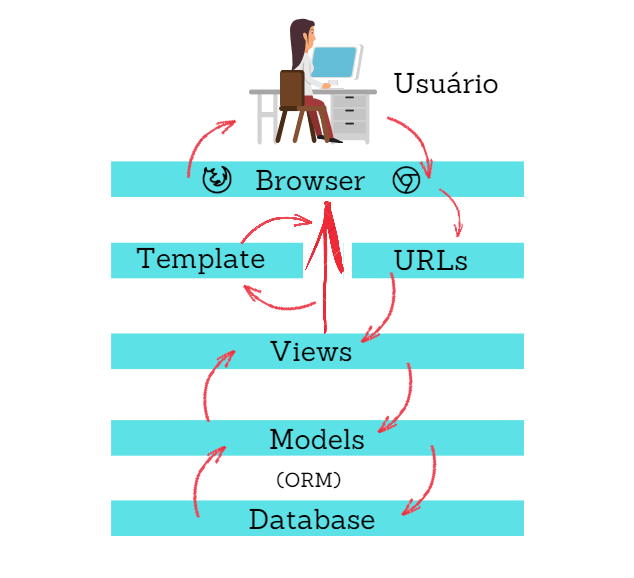
\includegraphics[width=0.85\textwidth]{Figuras/mvt-django.png}
    \caption*{Fonte: \cite{treinaweb2023mtv}}
    \label{fig:mtv}
\end{figure}

A diferença mais relevante entre os dois padrões está na forma como o roteamento de requisições é gerenciado. No MVC clássico, o \textit{Controller} é o ponto de entrada das requisições do cliente. No MTV do Django, esse papel é desempenhado pelo próprio mecanismo de roteamento de URLs do \textit{framework}, que mapeia cada endereço recebido para a \textit{View} correspondente por meio do arquivo \texttt{urls.py}, antes mesmo de qualquer lógica da aplicação ser acionada \cite{djangodocs}. A Figura~\ref{fig:mvc-vs-mtv} compara os dois padrões.

\begin{figure}[!htb]
    \centering
    \caption{Comparação entre as arquiteturas MVC e MTV}
    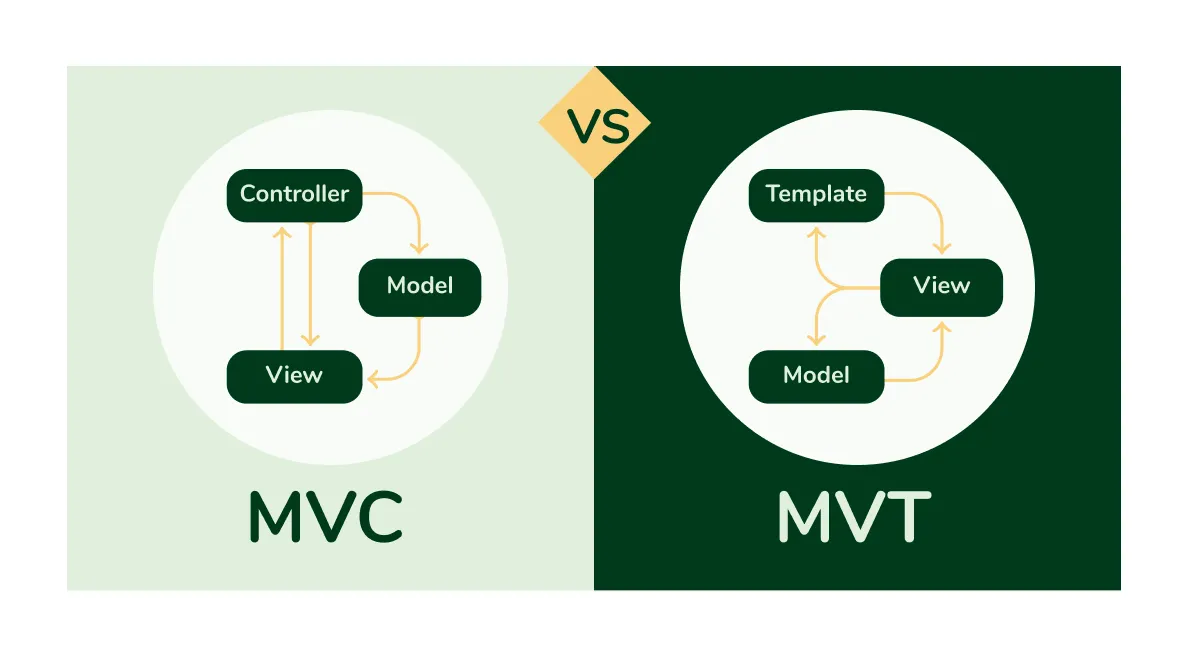
\includegraphics[width=0.85\textwidth]{Figuras/mvcVSmvt.png}
    \caption*{Fonte: \cite{djangodocs}}
    \label{fig:mvc-vs-mtv}
\end{figure}

O fluxo de uma requisição no Django, representado na Figura~\ref{fig:fluxo-mtv}, percorre essas camadas de forma sequencial: o cliente envia uma requisição HTTP, o roteador de URLs identifica a \textit{View} responsável, a \textit{View} acessa os \textit{Models} para obter ou persistir dados e, em seguida, seleciona o \textit{Template} adequado para gerar a resposta enviada de volta ao cliente \cite{silva2023mtv}.

\begin{figure}[!htb]
    \centering
    \caption{Fluxo de requisição na arquitetura MTV do Django}
    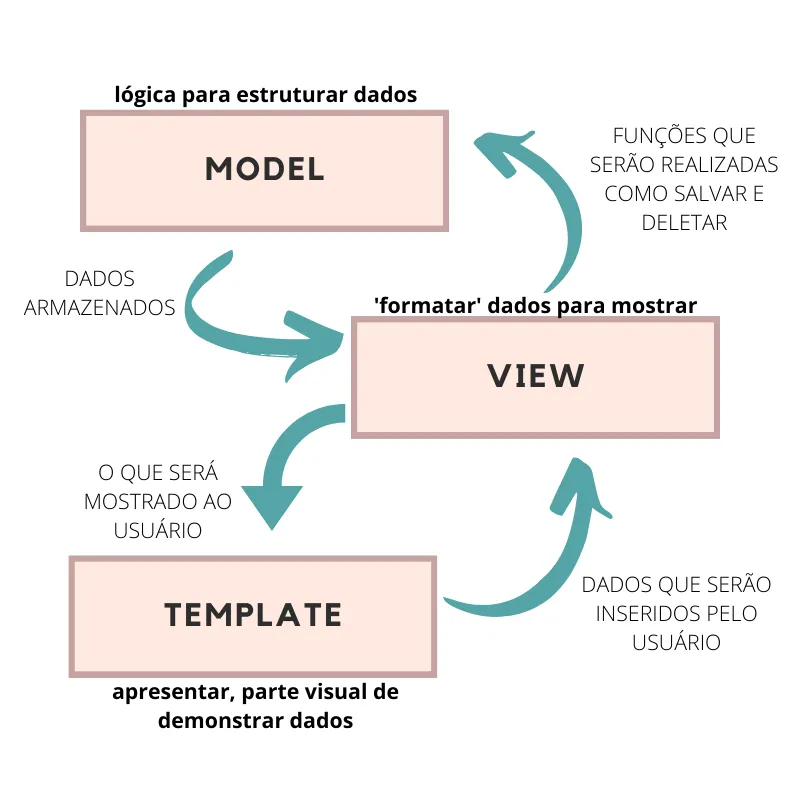
\includegraphics[width=0.85\textwidth]{Figuras/arquitetura.png}
    \caption*{Fonte: \cite{silva2023mtv}}
    \label{fig:fluxo-mtv}
\end{figure}

%-----------------------------------
\subsubsection{O Framework Django}
\label{sec:django}

O Django é um \textit{framework} web de código aberto escrito em Python. Seu conjunto de recursos inclui ORM, autenticação, roteamento de URLs, mecanismo de \textit{templates} e envio de e-mails, embora cada aplicação possa utilizar bibliotecas adicionais conforme suas necessidades \cite{djangodocs}. O \textit{framework} também segue o princípio \textit{Don't Repeat Yourself} (DRY), que orienta o reaproveitamento de código e a centralização de lógicas que, se duplicadas, aumentariam o custo de manutenção \cite{djangodocs}.

O roteamento de URLs é configurado no arquivo \texttt{urls.py}, que associa cada padrão de endereço a uma \textit{view} específica por meio da função \texttt{path()}. Quando uma requisição chega ao servidor, o \textit{framework} percorre a lista de padrões registrados até encontrar o primeiro que corresponda à URL solicitada e delega o processamento à \textit{view} associada. Esse mecanismo é independente da estrutura de diretórios da aplicação, o que permite organizar as URLs de forma legível e separada da lógica de negócio \cite{djangodocs}.

Cada \textit{model} do Django é uma classe Python que herda de \texttt{django.db.models.Model}. Cada atributo da classe representa uma coluna da tabela correspondente no banco de dados, e o tipo do campo, como \texttt{CharField}, \texttt{DateTimeField} ou \texttt{BooleanField}, determina o tipo de dado armazenado e as validações aplicadas \cite{djangodocs}. Relacionamentos entre entidades são representados por campos específicos: \texttt{ForeignKey} para associações muitos-para-um e \texttt{ManyToManyField} para associações muitos-para-muitos. O ORM traduz as operações sobre esses objetos Python em comandos SQL compatíveis com o banco de dados configurado \cite{djangodocs}.

As mudanças nos \textit{models} são controladas pelo sistema de \textit{migrations}. O comando \texttt{makemigrations} gera um arquivo descrevendo as alterações a serem aplicadas no banco; o comando \texttt{migrate} as aplica de forma incremental e rastreável, mantendo um histórico completo de todas as versões do esquema \cite{djangodocs}.

O sistema de \textit{templates} do Django utiliza a \textit{Django Template Language} (DTL), que insere dados dinâmicos nas páginas HTML por meio de variáveis e \textit{tags} de controle. Com a herança de \textit{templates}, obtida pelas \textit{tags} \texttt{\{\% extends \%\}} e \texttt{\{\% block \%\}}, um arquivo base define elementos comuns, como cabeçalho, menu e rodapé. Os demais arquivos sobrescrevem apenas os blocos específicos de cada página \cite{djangodocs}.

O Django inclui mecanismos de segurança que precisam ser habilitados e utilizados conforme a documentação. A proteção contra \textit{Cross-Site Request Forgery} (CSRF) usa um \textit{middleware} e o \textit{token} inserido pela \textit{tag} \texttt{\{\% csrf\_token \%\}} nos formulários. O sistema de \textit{templates} realiza escape automático do conteúdo dinâmico, reduzindo o risco de \textit{Cross-Site Scripting} (XSS) quando os mecanismos padrão não são desativados. Nas consultas feitas pelo ORM, os parâmetros são separados do comando SQL, o que reduz o risco de injeção; consultas SQL escritas manualmente ainda precisam seguir as práticas de segurança recomendadas \cite{djangodocs}.

%-----------------------------------
\subsubsection{Usabilidade e Interface do Usuário}
\label{sec:usab}

Usabilidade é a medida em que um produto pode ser usado por pessoas específicas para atingir objetivos específicos com eficácia, eficiência e satisfação num determinado contexto \cite{nielsen1993}. \citeonline{nielsen1993} descreve cinco atributos que compõem a usabilidade de um sistema: facilidade de aprendizado, eficiência de uso, facilidade de memorização, baixa taxa de erros e satisfação subjetiva do usuário. Um sistema com boa usabilidade permite que o usuário realize suas tarefas sem depender de treinamento extensivo nem de suporte constante.

Para orientar o projeto de interfaces, \citeonline{nielsen1994} propôs dez heurísticas de usabilidade que se tornaram referência na área: (1) visibilidade do estado do sistema, mantendo o usuário informado sobre o que está acontecendo; (2) correspondência entre o sistema e o mundo real, usando linguagem e convenções familiares ao usuário; (3) controle e liberdade do usuário, permitindo desfazer ações e sair de estados indesejados; (4) consistência e padrões, seguindo convenções da plataforma para que o usuário não precise aprender novos significados; (5) prevenção de erros, projetando para evitar que erros ocorram; (6) reconhecimento em vez de memorização, tornando objetos e opções visíveis para reduzir a carga de memória do usuário; (7) flexibilidade e eficiência de uso, permitindo que usuários experientes realizem tarefas mais rapidamente; (8) estética e design minimalista, evitando informações irrelevantes que competem com o conteúdo principal; (9) ajuda para reconhecer, diagnosticar e recuperar erros, exibindo mensagens claras sobre o que deu errado e como corrigir; e (10) ajuda e documentação, oferecendo suporte quando necessário, de forma fácil de buscar e orientada à tarefa.

Algumas dessas heurísticas têm peso particular no sistema proposto. A visibilidade do estado do sistema é importante porque o docente precisa saber, a qualquer momento, se a sua solicitação de reserva está pendente, aprovada ou rejeitada. A correspondência com o mundo real orienta o uso de termos como ``laboratório'', ``reserva'' e ``disponível'' em vez de jargões técnicos. A prevenção de erros, por sua vez, inclui mecanismos como a verificação automática de conflitos de horário antes de permitir a solicitação.

No contexto deste trabalho, usabilidade é relevante porque o sistema é destinado a docentes com familiaridade tecnológica variada. Um sistema que exija treinamento extensivo ou que gere dúvidas frequentes tende a ser abandonado, o que comprometeria o próprio objetivo de substituir o processo manual de agendamento.
%-----------------------------------
\subsubsection{Testes de Software}
\label{sec:testes}

Testes de software são atividades planejadas com o objetivo de verificar se um sistema se comporta conforme o esperado e identificar defeitos antes que o produto chegue ao usuário final. \citeonline{sommerville2018} define teste como um processo de validação e verificação que busca demonstrar que o software atende aos seus requisitos e identificar situações em que ele se comporta de forma incorreta ou inesperada. \citeonline{pressman2016} complementam essa perspectiva ao afirmar que testar é executar um programa com a intenção explícita de encontrar erros, distinguindo o processo de testes de outras atividades de garantia de qualidade por seu caráter sistematicamente verificativo: um teste bem-sucedido é aquele que revela um defeito até então desconhecido.

Os testes unitários são a forma mais elementar de teste de software e têm como foco verificar o comportamento de unidades individuais de código de forma isolada, antes de integrá-las ao restante do sistema. \citeonline{myers2011} definem teste unitário como o processo de testar subprogramas, funções ou métodos de maneira independente, de modo que, quando uma unidade falha, a localização do defeito seja imediata, sem a necessidade de investigar interações entre múltiplos componentes. \citeonline{pressman2016} acrescentam que os testes unitários devem cobrir as estruturas de controle internas de cada componente, as condições de contorno, os caminhos independentes de execução e o tratamento de erros.

No contexto de sistemas web com regras de negócio definidas, os testes unitários têm papel direto na validação da lógica da aplicação. \citeonline{sommerville2018} observa que os testes unitários são especialmente eficazes para validar componentes que implementam regras de negócio, pois permitem verificar cada condição individualmente e com precisão. À medida que as unidades validadas são combinadas, os testes de integração verificam se os componentes interagem corretamente entre si \cite{pressman2016}.

%---------------------------------
% SEÇÃO DE METODOLOGIA
%---------------------------------
